\chapter{System architecture}
\label{ch:model}

% As was shown in~\Cref{ch:problem}, the requirements are the following.
% \begin{itemize}
%     \item Global consensus
%     \item Security and fault tolerance
%     \item Performance and scalability
% \end{itemize}

% As mentioned in the Introduction, the primary goal is performance and scalability.
% Having a scalable blockchain system while still keeping global consensus
% allows the system to be ubiquitous and realise the full potential of blockchain.

% The secondary goal is to design an application neutral system.
% In particular, it should act as a backbone that provides the building blocks of blockchain based applications.
% It should be possible to buld any kind of application on top our system.
% Further, we do not impose on a consensus algorithm, as long as it satisfies the properties of atomic broadcast which we describe in~\Cref{sec:overview-cons}.


% The third and final goal is security.
% Our system should be unaffected in the presence of powerful adversaries.
% In particular, adversaries are Byzantine meaning that they can have arbitrary behaviour.
% Thus anything is possible from simply ommitting messages to colluding with eachother in order to undermine the whole system.

Our system consists of three protocols---the consensus protocol, the transaction protocol and the validation protocol.
It is based on our prior work on TrustChain~\cite{multichain},
where every node independently interacts with each other via their own blockchain\footnote{It is originally called MultiChain but the name has changed to TrustChain}.

The goal of this chapter is to detail our system specification.
We begin our discussion with an intuitive overview of the architecture in \Cref{sec:system-overview}.
Next, we give the formal description, starting with the model and assumptions in \Cref{sec:model-assumptions}.
Then, the three protocols which make up the complete system,
namely consensus protocol (\Cref{sec:cons-protocol}), transaction protocol (\Cref{sec:tx-protocol}) and validation protocol (\Cref{sec:vd-protocol}).
Finally, we discuss a few variations of our main design and their respective tradeoffs in \Cref{sec:tradeoffs}.

\section{System overview}
\label{sec:system-overview}
The architecture is visualised in~\Cref{fig:architecture}.
\begin{figure}[h]
\centering
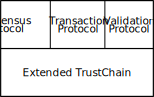
\includegraphics[width=0.7\textwidth]{architecture}
\caption{Overview of the system architecture}
\label{fig:architecture}
\end{figure}
It consists of one data structure---Extended TrustChain, and three protocols.
The protocols have distinct roles which are evident from their names.
They run concurrently and do not interact with each other.
The only synchronization happens on the Extended TrustChain layer, where all the protocols read and write from it.
We first describe each component individually, starting with Extended TrustChain, and then explain how they fit together.

\subsection{Extended TrustChain}
Extended TrustChain naturally builds on top of the standard TrustChain. 
Thus we first describe the standard TrustChain.
Our description has minor differences compared to the description in~\cite{multichain}.
This is to help with the description of the extended TrustChain.
We remark the difference when it occurs.
However, the two descriptions are functionally the same.

\subsubsection*{Standard TrustChain}
In TrustChain, every node has a ``personal'' chain. 
Initially, the chain only contains a genesis block generated by the nodes themselves.
When a node $A$ wishes to add a new transaction (TX) with $B$,
a new TX block is generated for both $A$ and $B$ and is appended to their respective chains.
The TX block must have a valid hash pointer pointing to the previous block
and a reference\footnote{This is different from the original TrustChain definition found in~\cite{multichain}.
In there, a TX block has two outgoing edges which are hash pointers to the two parties involved in the transaction.
This work uses one outgoing edge and a reference.} to its \emph{pair} on $B$'s chain.
An example of is shown in \Cref{fig:trustchain-bad}.

\begin{figure}
    \includegraphics[width=0.9\textwidth]{trustchain-bad}
    \centering
    \caption{Every block is denoted by $t_{i,j}$, where $i$ is the node ID and $j$ is the sequence number of the block.
    Thus we have three nodes and three corresponding chains in this example.
    The arrows represent hash pointers and the dotted lines represent references.
    The blocks at the ends of one dotted line are pairs of each other.
    The red block after $t_{b, 5}$ indicates a fork.}
    \label{fig:trustchain-bad}
\end{figure}

If every node follows the rules of TrustChain and we only consider hash pointers and not references,
then every chain effectively forms a singly linked list.
However, if a node violates the rules, then a \emph{fork} may happen.
That is, there may be more than one TX block with a hash pointer pointing back to the same block.
In \Cref{fig:trustchain-bad}, node $b$ (in the middle chain) created two TX blocks that both point to $t_{b, 5}$.
If this is a ledger system it can be seen as a double spend, where the currency accumulated up until $t_{b, 5}$ is spent twice.

\subsubsection*{Extended TrustChain}
We are now ready to explain the Extended TrustChain.
The primary difference is the introduction of a new type of block---checkpoint (CP) block.
In contrast to TX blocks, CP blocks do not store transactions or contain references.
Their purpose is to capture the state of the chain and the state of the whole system.
In particular, the state of the chain is captured with a hash pointer.
The state of the whole system is captured in the content of the CP block,
namely as a digest of the latest \emph{consensus result} which we explain in \Cref{sec:overview-cons}.
A visual representation is shown in \Cref{fig:trustchain-bad-cp}.

From this point on, we use TrustChain to mean the Extended TrustChain unless explicitly clarified.

\begin{figure}
    \includegraphics[width=0.9\textwidth]{trustchain-bad-cp}
    \centering
    \caption{The circles represent CP blocks,
    they also have hash pointers (arrow) but do not have references (dotted line).
    Note that the sequence number counter do not change, it is shared with TX blocks.}
    \label{fig:trustchain-bad-cp}
\end{figure}

\subsection{Consensus protocol}
\label{sec:overview-cons}

% The consensus protocol uses an existing Byzantine consensus algorithm (explained in detail in \Cref{sec:xyz}) and runs it continuously in rounds.
The consensus protocol can be seen as a technique of running infinitely many rounds of some 
Byzantine consensus algorithm\footnote{More accurately it is ACS or asynchronous subset consensus, we describe ACS in \Cref{sec:acs-background}.},
starting a new execution immediately after the previous one is completed.
This is necessary because blockchain systems always need to reach consensus on new values proposed by nodes in the system,
or CP blocks in our case.

The high communication complexity of Byzantine consensus algorithms prohibits us from running it on a large network.
Thus, for every round, we randomly select some node---called facilitators---to collect CP blocks from every other node and use them as the proposal.
The facilitators are elected using a \emph{luck value}, which is computed using $\textsf{H}(\C_r || pk_u)$,
where $\C_r$ is the consensus result 
(which can be seen as the set union of all the CP blocks collected by the facilitators)
in round $r$ and $pk_u$ is the public key of node $u$.
Intuitively, the election is guaranteed to be random 
because the output of a cryptographically secure hash function is unpredictable and $\C_r$ cannot be determined in advance.
Finally, the elected facilitators run a Byzantine consensus algorithm to agree on a set of CP blocks.
The next round begins when the new facilitators are computed from these CP blocks.

A visual explanation can be found in \Cref{app:consensus-example},
it walks through the steps needed for a node to be selected as a facilitator using an example.

\subsection{Transaction and validation}
The TX protocol is a simple request and response protocol.
The nodes exchange one round of messages and create new TX blocks on their respective chains.
Thus, as we mentioned before, one transaction should result in two TX blocks.

The consensus and transaction protocol by themselves do not provide a mechanism to detect tampering.
Thus we need a validation protocol to counteract malicious behaviour.
When a node wishes to validate one of its TX, it asks the counterparty for the \emph{agreed fragment} of the TX.
An agreed fragment of a TX block is a section of the chain beginning and ending with CP blocks that contain the TX block,
the CP blocks must also be in consensus.
Upon the counterparty's response, the node checks that the CP blocks are indeed in consensus,
the hash pointers are valid and his TX is actually in the fragment.
The TX is valid if these conditions are satisfied.
Intuitively, this works because it is hard (because a cryptographically secure hash function is second-preimage resistant)
to create a different chain that begins and ends with the same two CP blocks.


\subsection{Combined protocol}
\label{sec:combined-protocol}
The final result is essentially the concurrent composition of the three aforementioned protocols,
all making use the Extended TrustChain data structure.

Our sub-protocol design gives us the highly desirable non-blocking property.
In particular, we do not need to ``freeze'' the state of the chain for some communication to complete in order to create a block.
For instance, a node may start the consensus protocol, and while it is running, create new transactions and validate old transactions.
By the time the consensus protocol is done, the new CP block is added to whatever the state that the chain is in.
It is not necessary to lock the chain while the consensus protocol is running and then unlock it afterwards.

\section{Model and assumptions}
\label{sec:model-assumptions}

This section and the ones following it give a technical treatment of what the content in System overview.
For notational clarity, we use the following convention (adapted from~\cite{miller2016honey}) for most of this work.
\begin{itemize}
\item Lower case (e.g. $x$) denotes a scalar object or a tuple.
\item Upper case (e.g. $X$) denotes a set or a constant.
\item Sans serif (e.g. $\textsf{fn}(\cdot)$) denotes a function.
\item Monospace (e.g. $\texttt{ack}$) denotes message type.
\end{itemize}
Further, we use $a || b$ to denote concatenation of the binary representations of $a$ and $b$.

We assume purely asynchronous channels with eventual delivery.
Thus in no stage of our protocol do we make timing assumptions.
The adversary has full control of the delivery schedule and the message ordering of all messages.
But they are not allowed to drop messages except for their own\footnote{
    Reliability can be achieved in unreliable networks by resending messages or using some error correction code.
}.

We assume there exists a Public Key Infrastructure (PKI), and nodes are identified by their unique and permanent public key.
Finally, we use the random oracle (RO) model, i.e. calls to the random oracle are denoted by $\textsf{H}: \{0, 1\}^* \rightarrow \{0, 1\}^\lambda$,
where $\{0, 1\}^*$ denotes the space of finite binary strings and $\lambda$ is the security parameter.
Under the RO model, the probability of successfully computing the inverse of the hash function is negligible with respect to $\lambda$~\cite{bellare1993random}.

% TODO big N does not follow our convention
In our model, we consider $N$ nodes, which is the population size.
$n$ of them are facilitators, $t$ out of $n$ are malicious and the inequality
$n \ge 3t + 1$ must hold.
This is from the work of Pease, Shostak and Lamport, where they show a network of $n$ nodes cannot reach Byzantine agreement with $t \ge n/3$~\cite{pease1980reaching}.
Further, the inequality $N \ge n + t$ must also hold.
This is due to our system design, which becomes clear in~\Cref{sec:consensus-phase}.

Our threat model is as follows. 
We use a restricted version of the adaptive corruption model.
The first restriction is that corrupted node can only change across rounds.
That is, if a round has started, the corrupted nodes cannot change until the next round.
The second restriction is that the adversary, presumably controlling all the corrupted nodes, is forgetful.
Namely, the adversary may learn the internal state such as the private key of a corrupted node,
but if the node recovers, then the adversary must forget the private key.
This is realistic because otherwise the adversary can eventually learn all the private keys and sabotage the system.

\section{Extended TrustChain}
The primary data structure used in our system is the Extended TrustChain.
Each node $u$ has a public and private key pair---$pk_u$ and $sk_u$, and a chain $B_u$.
The chain consist of blocks $B_u = \{ b_{u, i} : i \in \{ 0, \dots, h - 1 \} \}$,
where $b_{u, i}$ is the $i$th block of $u$,
and $h$ is the height of the block (i.e. $h = |B_u|$).
We often use $b_{u, h}$ to denote the latest block.
There are two types of blocks, TX blocks and CP blocks.
If $T_u$ is the set of all TX blocks in $B_u$ and $C_u$ is the set of all CP blocks is $B_u$,
then it must be the case that $T_u \cup C_u = B_u$ and $T_u \cap C_u = \varnothing$.
The notation $b_{u, i}$ is generic over the block type.
We assume there exists a function $\textsf{typeof}: B_u \rightarrow \{ \tau, \gamma \}$ that returns the type of the block,
where $\tau$ represents the TX type and $\gamma$ represents the CP type.

\begin{definition}
\textbf{\emph{Transaction block}}

The TX block is a six-tuple, i.e $t_{u, i} = \langle \textsf{H}(b_{u, i - 1}), seq_u, txid, pk_v, m, sig_u \rangle$.
We describe each item in turn.
\begin{enumerate}
\item $\textsf{H}(b_{u, i - 1})$ is the hash pointer to the previous block.
\item $seq_u$ is the sequence number which should equal $i$.
\item $txid$ is the transaction identifier, it should be generated using a cryptographically secure pseudo-random number generator by the initiator of the transaction.
\item $pk_v$ is the public key of the counterparty $v$.
\item $m$ is the transaction message.
\item $sig_u$ is the signature created using $sk_u$ on the concatenation of the binary representation of the five items above.
\end{enumerate}
The fact that we have no constraint on the content of $m$ is in alignment with our design goal---application neutrality.

TX blocks come in pairs.
In particular, for every block 
$$t_{u, i} = \langle \textsf{H}(b_{u, i - 1}), seq_u, txid, pk_v, m, sig_u \rangle$$
there exist one and only one \emph{pair} 
$$t_{v, j} = \langle \textsf{H}(b_{v, j - 1}), seq_v, txid, pk_u, m, sig_v \rangle.$$
Note that the $txid$ and $m$ are the same, and the public keys refer to each other.
Thus, given a TX block, these properties allow us to identify its pair.
\end{definition}

% TODO Node $v$ may cheat and create more than one pair for $t_{u, i}. we discuss later

\begin{definition}
\textbf{\emph{Checkpoint block}}

The CP block is a five-tuple, 
i.e. $c_{u, i} = \langle \textsf{H}(b_{u, i-1}), seq_u, \textsf{H}(\C_r), r, sig_u \rangle$,
where $\C_r$ is the consensus result (which we describe in \Cref{sec:consensus-result}) in round $r$, the other items are the same as the TX block definition.
% Note that unlike in our prior work~\cite{implicitconsensus}, CP blocks and TX blocks do not have independent sequence numbers.

The genesis block in the chain must be a CP block in the form of
$c_{u, 0} = \langle \textsf{H}(\bot), 0,  \textsf{H}(\bot), 0, sig_u \rangle$
where $\textsf{H}(\bot)$ can be interpreted as applying the hash function on an empty string.
The genesis block is unique because every node has a unique public and private key pair.
\end{definition}


\begin{definition}
\label{sec:consensus-result}
\textbf{\emph{Consensus result}}

Our consensus protocol runs in rounds as discussed in \Cref{sec:system-overview}.
Every round is identified by a round number $r$, which is incremented on every new round.
The consensus result is a tuple, i.e. $\C_r = \langle r, C \rangle$,
where $C$ is a set of CP blocks agreed by the facilitators of round $r$.
\end{definition}

Here we define an important property which results from the interleaving nature of CP and TX blocks.
It is used in our validation protocol.
\begin{definition}
\textbf{\emph{Enclosure and agreed enclosure}}

If there exist a tuple $\langle c_{u,a}, c_{u, b} \rangle$ for a TX block $t_{u, i}$,
where 
$$a = \argmin_{k, k < i, \texttt{typeof}(b_{u,k}) = \gamma}(i - k)$$
$$b = \argmin_{k, k > i, \texttt{typeof}(b_{u,k}) = \gamma}(k - i),$$
then $\langle c_{u,a}, c_{u, b} \rangle$ is the enclosure of $t_{u, i}$.
Intuitively, that is the two closest CP blocks that surround $t_{u, i}$.
Note that $c_{u, a}$ is the more recent CP block.
Also, some TX blocks may not have any enclosure, then its enclosure is $\bot$.
Agreed enclosure is the same as enclosure with an extra constraint where the CP blocks must be in some consensus result $\C_r$.

\end{definition}

Note that the ``closest CP blocks'' property must also apply to agreed enclosure. 
Suppose a chain is in the form
$\{c_{i}, c_{i+1}, t_{i+2}, c_{i+3}\}$\footnote{Usually the notation is of the form $c_{u, i}$, but the node identity is not important here so we simplify it to $c_{i}$}
and $c_{i}, c_{i+1}, c_{i+3}$ are in $\C_r, \C_{r+1}, \C_{r+3}$ respectively,
then the agreed enclosure of $t_{i+2}$ is $\langle c_{i+1}, c_{i+3}\rangle$ and cannot be $\langle c_{i}, c_{i+3}\rangle$.

\begin{definition}
\textbf{\emph{Fragment and agreed fragment}}

If the enclosure of some TX block $t_{u, i}$ is $\langle c_{u,a}, c_{u, b} \rangle$,
then its \emph{fragment} $F_{u, i}$ is defined as $\{ b_{u, i} : a \le i \le b \}$.
Similarly, \emph{agreed fragment} has the same definition as fragment but using agreed enclosure.
For convenience, the function $\textsf{agreed\_fragment}(\cdot)$ represents the agreed fragment of some TX block if it exists, otherwise $\bot$.
\end{definition}

% The length of the fragment is constrained by $L$,
% namely $\forall t |\textsf{fragment}(t)| \le L$.
% The purpose to prevent spam and encourage nodes to create more CP blocks.
% $L$ should be sufficiently high so that busy nodes are not hindered by it.

\section{Consensus protocol}
\label{sec:cons-protocol}

Our scalable consensus protocol runs on top of Extended TrustChain.
It uses an unmodified asynchronous subset consensus (ACS) algorithm as the key building block.
The objectives of the protocol are to
    allow honest nodes always make progress (in the form of creating new CP blocks),
    compute correct consensus result in every round
    and have an unbiased election of facilitators.
Concretely, we define the necessary properties as follows.
\begin{definition}
\label{def:consensus}
\textbf{\emph{Properties of the consensus protocol}}

$\forall r \in \mathbb{N}$, the following properties must hold.
\begin{enumerate}
    \item \emph{Agreement}:
        If one correct node outputs a set of facilitators $\F_r$,
        then every node outputs $\F_r$
    \item \emph{Validity}:
        If any correct node outputs $\F_r$, then 
            \begin{enumerate}
                \item $|\C_r| \ge N - t$ and each CP in $\C_r$ belong to a different node\footnote{
                $\C_r$ is a tuple but we abuse the notation here by writing $|\C_r|$ to mean the number of CP blocks in the second element of $\C_r$.}.
                \item $\F_r$ must contain at least $n - t$ honest nodes and
                \item $|\F_r| = n$.
            \end{enumerate}
    \item \emph{Fairness}:
        Every node with a CP block in $\C_r$ should have an equal probability of becoming a member of $\F_r$.
    \item \emph{Termination}:
        Every correct node eventually outputs some $\F_r$.
\end{enumerate}
\end{definition}
These properties may look like Byzantine consensus properties (which we describe next in \Cref{sec:acs-background}) but there are subtle differences.
Firstly, they are properties for every node in the network and not just the facilitators.
Secondly, they must be satisfied for all rounds because the whole system falls apart if one of the property cannot be satisfied in one of the rounds.

Before describing the protocol in detail,
we take a brief detour to give background on the ACS algorithm as it is the primary building block.
Then we move on to describe the two phases of our consensus protocol---bootstrap phase and consensus phase.

\subsection{Background on asynchronous subset consensus}
\label{sec:acs-background}

The best way to explain ACS is to contrast it with the typical Byzantine consensus.
We adapt the description from~\cite[Chapter 17]{podc}.
%The Byzantine consensus problem is a classical problem is distributed systems literature.
%It is first described by Leslie Lamport as the Byzantine general's problem in 1982~\cite{lamport1982byzantine}.
%Byzantine consensus is described as follows (adapted from ).
\begin{definition}
\textbf{\emph{Byzantine consensus}}

There are $n$ nodes, of which at most $t$ might experience Byzantine fault.
Node $i$ starts with an input value $v_i$.
The nodes must decide for one of  those values, satisfying the following.
\begin{enumerate}
    \item \emph{Agreement:}
        If a correct node outputs $v$, then every node outputs $v$.
    \item \emph{Validity:}
        The decision value must be the input value of a node.
    \item \emph{Termination:}
        All correct nodes terminate in finite time.
\end{enumerate}
\end{definition}
A node under Byzantine fault means that it can have arbitrary behaviour.
For example not sending a message or colluding with other Byzantine nodes to undermine the entire system.
Note that the decision is on a single value.
This is in contrast to ACS which we describe next.

ACS is an especially useful primitive for blockchain systems.
It allows any party to propose a value and the result is the set union of all the proposed values by the majority.
Concretely, ACS needs to satisfy the following properties (adapted from~\cite{miller2016honey}).
\begin{definition}
\label{def:acs}
\textbf{\emph{Asynchronous subset consensus}}

There are $n$ nodes, of which at most $t$ might experience Byzantine fault.
Node $i$ starts with a non-empty set of input values $C_i$.
The nodes must decide an output $C$, satisfying the following.
\begin{enumerate}
    \item \emph{Agreement:}
        If a correct node outputs $C$, then every node outputs $C$.
    \item \emph{Validity:}
        If any correct node outputs a set $C$,
        then $|C| \ge n - t$ and $C$ contains the input of at least $n - 2t$ nodes.
    \item \emph{Totality:}
        If $n - t$ nodes receive an input, then all correct nodes produce an output.
\end{enumerate}
\end{definition}

ACS has the nice property of censorship resilience when compared to other consensus algorithms.
For instance, Hyperledger and Tendermint uses a variant of Practical Byzantine Fault Tolerance (PBFT)~\cite{castro1999practical} as their consensus algorithm.
In PBFT, a leader is elected, if the leader is malicious but follows the protocol, then it can selectively filter transactions.
In contrast, every party in ACS are involved in the proposal phase,
and it guarantees that if $n - 2t$ parties propose the same transaction, then it must be in the agreed output.
Thus, if some value is submitted to at least $n - 2t$ nodes, it is guaranteed to be in the consensus result.
For a detailed description of ACS, we refer to the HoneyBadgerBFT work~\cite{miller2016honey}.
To understand the remainder of this work, the knowledge of~\Cref{def:acs} is sufficient.

The main drawback with ACS and also Byzantine consensus algorithms is the high message complexity.
Typically, such protocols have a message complexity of $O(n^2)$, where $n$ is the number of parties.
Hence, it may work with a small number of nodes,
but it is infeasible for blockchain systems where thousands of nodes are involved.

% The literature on Byzantine consensus and atomic broadcast is rich, some noteable ones include TODO.
% Thus in the ETC consensus protocol, we assume there exist an "off-the-shelf" Byzantine consensus algorithm which we can use
% (in our implementation we use HoneyBadgerBFT and motivate our choice in TODO).

% In our case, every node do not propose some arbitrary data, but a set of CP blocks.
% Thus the result of the consensus is the set union of all the legitimate proposals.


\subsection{Bootstrap phase}
\label{sec:bootstrap}
Now we have all the necessary information to describe our consensus protocol.
As with all distributed systems, there must be a bootstrap phase which sets up the system.

The reader may notice from the system overview (\Cref{sec:system-overview}) that the facilitators are computed from the consensus result,
but the consensus result is agreed by the facilitators.
Thus we have a dependency cycle.
The goal of the bootstrap phase is to give us a starting point in the cycle.

To bootstrap, imagine that there is some bootstrap oracle, that initiates the code on every node.
The code satisfies all the properties in \Cref{def:consensus}.
Namely, every node has the same set of valid facilitators $\F_1$ that are randomly chosen.
This concludes the bootstrap phase.
For any future rounds, the consensus phase is used.

In practice, the bootstrap oracle is most likely the software developer and some of the desired properties cannot be achieved.
In particular, it is not possible to have the fairness property because it is unlikely that the developer knows the identity of every node in advance.

\subsection{Consensus phase}
\label{sec:consensus-phase}
The consensus phase begins when $\F_r$ is available to all the nodes.
Note that $\F_r$ indicates the facilitators that were elected using results of round $r$ and are responsible for driving the ACS protocol in round $r + 1$.
The goal is to reach agreement on a set of new facilitators $\F_{r + 1}$ that satisfies the four properties in \Cref{def:consensus}.

There are two scenarios in the consensus phase.
First, if node $u$ is not the facilitator, it sends $\langle \texttt{cp\_msg}, c_{u, h} \rangle$ to all the facilitators.
Second, if the node is a facilitator, it waits until $N - t$ messages of type \texttt{cp\_msg} are received.
% Second if the node is a facilitator, it waits for some duration $D$ and collect messages of type \texttt{cp\_msg}, where $D \gg \Delta$.
Invalid messages are removed.
That is blocks with invalid signatures and blocks signed by the same key.
With the sufficient number of \texttt{cp\_msg} messages,
it begins the ACS algorithm and some $\C'_{r + 1}$ should be agreed upon by the end of it.
Duplicates and blocks with invalid signatures are again removed from $\C'_{r+1}$ and we call the final result $\C_{r+1}$.
We have to remove invalid blocks a second time (after ACS) because the adversary may send different CP blocks to different facilitators,
which results in invalid blocks in the ACS output, but not in any of the inputs.

The core of the consensus phase is the ACS protocol.
While any ACS protocol that satisfies the standard definition will work,
we use a simplification of HoneyBadgerBFT~\cite{miller2016honey} as our ACS protocol
because it is a consensus algorithm designed for blockchain systems.
We do not use the full HoneyBadgerBFT due to the following.
First, the transactions in HoneyBadgerBFT are first queued in a buffer and the main consensus algorithm starts only when the buffer reaches an optimal size.
We do not have an infinite stream of CP blocks, thus buffering is unsuitable.
Second, HoneyBadgerBFT uses threshold encryption to hide the content of the transactions.
But we do not reach consensus on transactions, only CP blocks, so hiding CP blocks is meaningless for us as it contains no transaction information.

Continuing, when $\F_{r}$ reaches agreement on $\C_{r+1}$,
they immediately broadcast two messages to all the nodes---
first the consensus message $\langle \texttt{cons\_msg}, \C_{r+1} \rangle$,
and second the signature message $\langle \texttt{cons\_sig}, r, sig \rangle$.
The reason for sending \texttt{cons\_sig} is the following.
Recall that channels are not authenticated, 
and there are no signatures in $\C_{r + 1}$.
If a non-facilitator sees some $\C_{r + 1}$, it cannot immediately trust it because it may have been forged.
Thus, To guarantee authenticity, every facilitator sends an additional message that is the signature of $\C_{r + 1}$.

Upon receiving $\C_{r + 1}$ and at least $n - f$ valid signatures by some node $u$, $u$ performs two tasks.
First, it creates a new CP block using $\textsf{new\_cp}(\C_{r + 1}, r + 1)$ using \Cref{alg:new-cp}.
Second, it computes the new facilitators using $\textsf{get\_facilitator}(\C_{r + 1}, n)$ using \Cref{alg:facilitator},
and updates its facilitator set to the result.
This concludes the consensus phase and brings us back to the beginning of the consensus phase.

\begin{algorithm}
\caption{Function $\textsf{new\_cp}(\C_r, r)$ runs in the context of the caller $u$.
It creates a new CP block and appends it to $u$'s chain.}
\label{alg:new-cp}
\begin{algorithmic}
\State $h \gets |B_u|$
\State $c_{u, h} \gets \langle \textsf{H}(b_{u, h-1}), h, \textsf{H}(\C_r), r, sig_u \rangle$
\State $B_u \gets B_u \cup c_{u, h}$
\end{algorithmic}
\end{algorithm}

\begin{algorithm}
\caption{Function $\textsf{get\_facilitator}(\C_r, n)$ takes the consensus result $\C_r$ and an integer $n$,
then sorts the CP blocks $C$ by the luck value (the $\lambda$-expression), and outputs the smallest $n$ elements.}
\label{alg:facilitator}
\begin{algorithmic}
\State $\langle r, C \rangle \gets \C_r$
\State $\textsf{take} (n, \textsf{sort\_by} (\lambda x.\textsf{H}(\C_r || pk \text{ of } x), C))$
\end{algorithmic}
\end{algorithm}


Our protocol has some similarities with synchronizers~\cite[Chapter 10]{podc} because it is effectively a technique to introduce synchrony in an asynchronous environment.
If we consider the facilitators as a collective authority, then it can be seen as a synchronizer that sends pulse messages (in the form of \texttt{cons\_msg} and \texttt{cons\_sig}) to indicate the start of a new clock pulse.
Every node then sends a completion messages (in the form of \texttt{cp\_msg}) to the new collective authority to indicate that they are ready for the next pulse.


\section{Transaction protocol}
\label{sec:tx-protocol}

The TX protocol, shown in \Cref{alg:tx-proto}, is run by all nodes.
It is also known as True Halves, first described by Veldhuisen~\cite[Chapter~3.2]{truehalves}.
Nodes that wish to initiate a transaction calls $\textsf{new\_tx}(pk_v, m, txid)$ (\Cref{alg:new-tx}) with the intended counterparty $v$ identified by $pk_v$ and message $m$.
$txid$ should be a uniformly distributed random value, i.e. $txid \in_R \{0, 1\}^{256}$.
Then the initiator sends $\langle \texttt{tx\_req}, t_{u, h}\rangle$ to $v$.

\begin{algorithm}
    \caption{Function $\textsf{new\_tx}(pk_v, m, txid)$ generates a new TX block and appends it to the caller $u$'s chain.
    It is executed in the private context of $u$, i.e. it has access to the $sk_u$ and $B_u$.
    The necessary arguments are the public key of the counterparty $pk_v$, the transaction message $m$ and the transaction identifier $txid$.}
    \label{alg:new-tx}

    \begin{algorithmic}
    \State $h \gets |B_u|$
    \State $t_{u, h} \gets \langle \textsf{H}(b_{u, h - 1}), h, txid, pk_v, m, sig_u \rangle$
    \State $B_u \gets B_u \cup \{ t_{u, h} \}$
    \end{algorithmic}
\end{algorithm}

\begin{algorithm}
    \caption{The TX protocol which runs in the context of node $u$.}
    \label{alg:tx-proto}

    \begin{algorithmic}
        \Upon $\langle \texttt{tx\_req}, t_{v, j} \rangle$ from $v$
        \State $\langle \_, \_, txid, pk_v, m, \_ \rangle \gets t_{v, j}$
        \State $\textsf{new\_tx}(pk_u, m, txid)$
        \State store $t_{v, j}$ as the pair of $t_{u, h}$
        \State send $\langle \texttt{tx\_resp}, t_{u, h} \rangle$ to $v$

        \Upon $\langle \texttt{tx\_resp}, t_{v, j} \rangle$ from $v$
        \State $\langle \_, \_, txid, pk_v, m, \_ \rangle \gets t_{v, j}$
        \State store $t_{v, j}$ as the pair of the TX with identifier $txid$
    \end{algorithmic}
\end{algorithm}

A key feature of the TX protocol is that it is non-blocking.
At no time in \Cref{alg:new-tx} or \Cref{alg:tx-proto} do we need to hold the chain state and wait for some message to be delivered before committing a new block to the chain.
This allows for high concurrency where we can call $\textsf{new\_tx}(\cdot)$ multiple times without waiting for the corresponding \texttt{tx\_resp} messages.

\section{Validation protocol}
\label{sec:vd-protocol}

Up to this point, we do not provide a mechanism to detect tampering.
The validation protocol aims to solve this issue.
The protocol is also a request-response protocol, just like the transaction protocol.
But before explaining the protocol itself, we first define what it means for a transaction to be valid.

\subsection{Validity definition}
A transaction can be in one of three states in terms of validity---\emph{valid}, \emph{invalid} and \emph{unknown}.
Given a fragment $F_{v, j}$, the validity of the TX block $t_{u, i}$ and the agreed fragment of it is captured by the function $\textsf{get\_validity}(t_{u, i}, F_{u, i}, F_{v, j})$ (\Cref{alg:get-validity}).
Note that $t_{u, i}$ and $F_{u, i}$ are assumed to be valid,
otherwise the node calling the function would have no point of reference.
This is not difficult to achieve.
Typically the caller is $u$, so it knows its own TX block and the corresponding agreed fragment.
If the caller is not $u$, it can always query for the agreed fragment that contains the transaction of interest from $u$.

\Cref{alg:get-validity} works as follows.
Before~\Cref{line:valid-fragment},
we essentially check whether the fragment is the one that the verifier needs.
If it is not, then the verifier cannot make any decision and return \emph{unknown}.
This is likely to be the case for new transactions because the result of $\textsf{agreed\_fragment}(\cdot)$ would be $\bot$.
The next two conditions check for tampering or missing blocks, if any of these misconducts are detected, then the TX is invalid.

We stress that the \emph{unknown} state means that the verifier does not have enough information to continue with the validation protocol.
If enough information is available at a later time, then the verifier will output either \emph{valid} or \emph{invalid}.

Note that the validity is on a transaction (two TX blocks with the same $txid$), rather than on one TX block owned by a single party.
It is defined this way because the malicious sender may create new TX blocks in their own chain but never send \texttt{tx\_req} messages.
In that case, it may seem that the counterparty, who is honest, purposefully omitted TX blocks.
But in reality, it was the malicious sender who did not follow the protocol.
Thus, in such cases, the whole transaction identified by its $txid$ is marked as invalid.

Further, the caller of $\textsf{get\_validity}(t_{u, i}, F_{u, i}, F_{v, j})$ is not necessarily 
$u$\footnote{In practice, it often is because after completing the TX protocol the parties are incentivised to check that the counterparty ``did the right thing''.}
Any node $w$ may call $\textsf{get\_validity}(t_u{u, i}, F_{u, i}, F_{v, j})$ as long as $w$ has an the necessary input parameters.
$F_{u, i}$  and $t_{u, i}$ may be readily available if $w = u$.
Otherwise, $w$ could query $u$ with the \texttt{vd\_req} message and then obtain the result from \texttt{vd\_resp}.
This is the validation protocol which we describe next.

\begin{algorithm}
\caption{Function $\textsf{get\_validity}(t_{u, i}, F_{u, i}, F_{v, j})$ validates the transaction represented by $t_{u, i}$.
We assume $F_{u, i}$ is always correct and contains $t_{u, i}$.
$F_{v, j}$ is the corresponding fragment received from $v$.}
\label{alg:get-validity}

\begin{algorithmic}[1]

    \If{$F_{v, j}$ is not a fragment created in the same round as $F_{u, i}$}
        \State \Return \emph{unknown}
    \EndIf
    \State

    \label{line:valid-fragment}
    \State $\langle \_, \_, txid, pk_v, m, \_ \rangle \gets t_{u, i}$
    \If{number of blocks of $txid$ in $F_{v, j} \ne 1$}
        \State \Return \emph{invalid}
    \EndIf
    \State

    \State $t_{v, j} \gets $ the TX block with $txid$ in $F_{v, j}$
    \State $\langle \_, \_, txid', pk_u, m', \_ \rangle \gets t_{v, j}$ 

    % message tampering
    \If{$m \ne m' \vee txid \ne txid'$} 
        \State \Return \emph{invalid}
    \EndIf
    \State

    % signature tampering
    \If{$t_{u, i} \text{ is not signed by } pk_u \vee t_{v, j} \text{ is not signed by } pk_v $}
        \State \Return \emph{invalid}
    \EndIf
    \State \Return \emph{valid}
\end{algorithmic}
\end{algorithm}

\subsection{Validation protocol}
Our validation protocol,
shown in~\Cref{alg:vd-proto},
is designed to classify transactions according to the aforementioned validity definition.
If $u$ wishes to validate some TX with ID $txid$ and counterparty $v$, it sends $\langle \texttt{vd\_req}, txid \rangle$ to $v$.
The desired properties of the validation protocol are as follows.
\begin{definition}
\label{def:validation}
\textbf{\emph{Properties of the validation protocol}}

\begin{enumerate}
    \item \emph{Agreement}:
        If any correct node decides on the validity (except when it is \emph{unknown}) of a transaction,
        then all other correct nodes are able to reach the same conclusion or \emph{unknown}.
    \item \emph{Validity}:
        The validation protocol outputs the correct result
        according to the aforementioned validity definition.
    % \item \emph{Unforgeability}:
    %     If some transaction is valid, it cannot be forged into an invalid transaction.
    %     If some transaction is invalid, it cannot be forged into a valid transaction.
    \item \emph{Liveness}:
        Any valid (invalid) transaction is marked as valid (invalid) eventually.
\end{enumerate}
\end{definition}

\begin{algorithm}
\caption{Validation protocol which runs in the context of $u$}
\label{alg:vd-proto}

\begin{algorithmic}
    \Upon $\langle \texttt{vd\_req}, txid \rangle$ from $v$
        \State $t_{u, i} \gets \text{the transaction identified by } txid$
        \State $F_{u, i} \gets \textsf{agreed\_fragment}(t_{u, i})$
        \State send $\langle \texttt{vd\_resp}, txid, F_{u, i} \rangle$ to $v$

    \Upon $\langle \texttt{vd\_resp}, txid, F_{v, j} \rangle$ from $v$
        \State $t_{u, i} \gets \text{the transaction identified by } txid$
        \If{$F_{u, i}$ and $F_{v, j}$ are available and $F_{u, i}$ is the agreed fragment of $t_{u, i}$}
            \State set the validity of $t_{u, i}$ to $\textsf{get\_validity}(t_{u, i}, F_{u, j}, F_{v, j})$
        \EndIf
\end{algorithmic}
\end{algorithm}

We make two remarks.
First, just like the TX protocol, we do not block at any part of the protocol.
Second, suppose some $F_{v, j}$ validates $t_{u, i}$, then that does not imply that $t_{u, i}$ only has one pair $t_{v, j}$.
Our validity requirement only requires that there is only one $t_{v, j}$ in the correct consensus round.
The counterparty may create any number of fake pairs in later consensus rounds.
But these fake pairs only pollutes the chain of $v$ and can never be validated because the round is incorrect.

\section{Design variations and tradeoffs}
\label{sec:tradeoffs}

Up to this point,
we have discussed our protocol in the context of the model and assumptions defined in \Cref{sec:model-assumptions}.
In this section, 
we explore a few design variations which we can make, some of them require a relaxed version of our original model.
They enable better performance, allow us to apply our design in the fully permissionless setting and improves privacy.

\subsection{Using epidemic protocol to reduce communication cost}
One of the final steps in our consensus protocol is to broadcast the consensus result and signatures to every other node (\Cref{sec:consensus-phase}).
While this guarantees delivery (since we assumed reliable channel), it is wasteful.
For example, if every facilitator is honest, a node would receive $n$ consensus results which are identical when only one is necessary.
Furthermore, realistic networks do not offer a broadcast primitive,
i.e. firewalls may block incoming messages from certain nodes.

An improvement is use an epidemic protocol~\cite{eugster2004epidemic} (also known as gossiping) instead of our broadcast approach.
Typical epidemic protocols works as follows.
Every node buffers every message it receives up to some buffer size $b$.
Then it forwards the messages $t$ number of times.
Every time the message is sent to $f$ random neighbours, $f$ is often called the fan-out.
The upside of using epidemic protocol is that the communication cost is distributed more evenly between nodes.
This is especially true with a lazy push approach where the node who just received a message would push the message ID (e.g. digest) to its $f$ random neighbours,
and only push the full message if the neighbour explicitly requests the message~\cite{leitao2007epidemic}.
With this, nodes typically only need to receive one consensus result message instead of $n$.

A down side of an epidemic protocol is that it usually takes $O(\log N)$ time to infect the whole network,
whereas broadcasting uses constant time.
Another downside of some epidemic protocols (e.g. eager push) is that it is difficult to guarantee delivery.
It is especially true when the parameters are not chosen correctly in a network that is only partially connected (but every node is nevertheless reachable).
If the delivery cannot be guaranteed, 
then we cannot guarantee liveness in our consensus protocol because a future facilitator may miss the memo.
Picking parameters are difficult in practice because the network configuration is unknown and the total number of nodes might also be unknown.


\subsection{Using timing assumption in the permissionless setting}
\label{sec:permissionless}
Our model is purely asynchronous, where we make no timing assumptions anywhere in the protocol.
However, in many applications it is often fine to make timing assumptions.
For example, TCP relies on timeout for its retransmission and the \texttt{nLockTime} property in Bitcoin transactions makes the transaction unspendable until some time in the future (either Unix time or block height)~\cite{bitcoindevguide}.
One limitation of our system is that we use the parameter $N$ in our algorithms, which makes it unsuitable for the permissionless environment where users can join and leave at will.
In this section we show how making a timing assumption would allow us to operate in the permissionless setting.

At the start of our consensus phase (\Cref{sec:consensus-phase}), facilitators must wait for $N-f$ \texttt{cp\_msg} messages.
This is the only place where we used $N$ as a parameter.
To introduce timing, instead of waiting for $N-f$ messages, we wait for some time $D$,
such that $D$ is sufficiently long for honest nodes to send their CP blocks to the facilitators.
Consequently, this removes the need for a PKI because the collected CP blocks may be from nodes that nobody has seen in the past.
However, choosing the parameter $D$ is difficult and depends on a number of factors such as the network condition, message size, and so on.
Overestimating it would make agreed fragments much longer than usual, which increases communication costs for validation.
Underestimating it would lead to unfairness where users with a poor internet connection will have a lower chance to be selected as a facilitator in the next round.
Nevertheless, there is a significant gain for making the timing assumption and that is the ability to operate in the permissionless setting which we explain next.

Suppose a new node wish to join the network and the facilitators are known (this can be done with a public registry).
It simply sends its latest CP block to the facilitators.
Then, in the next round, the node will have a chance to become a facilitator just like any existing node.
To leave the network, nodes simply stop submitting CP blocks.
There is a subtlety here which happens when the node is elected as a facilitator in the following round.
In this case, the node must fulfil its obligation by completing the consensus protocol, but without proposing its own CP block, before leaving.
Otherwise, the $n \ge 3t + 1$ condition may be violated.

\subsection{Privacy preserving validation protocol using compact blocks}
\label{sec:compact}
Our approach already has privacy preserving features in comparison to early blockchain systems.
That is, the transactions for each node are only revealed during the validation protocol.
Hence if two nodes never directly or indirectly interact with each other,
their transactions are never revealed.

We can take our privacy-preserving property one step further by introducing another level of hash pointer indirection.
The result is shown in~\Cref{fig:compact}.
\begin{figure}
    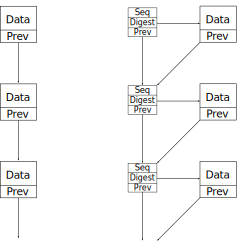
\includegraphics[width=0.7\textwidth]{compact}
    \centering
    \caption{The chain on the left represent direct chaining, where the digest in ``Prev'' is simply the digest of the previous block.
    The chain on the right uses compact blocks, represented by the smaller squares.
    Compact blocks also form a chain as before, but they each have a hash pointer to the full block, identified by ``Seq'' and ``Digest''.}
    \label{fig:compact}
\end{figure}

Concretely, we introduce an additional block type,
namely compact block.
Such blocks only have three attributes,
\begin{enumerate}
\item Seq---the sequence number its corresponding block,
\item Digest---the digest of its corresponding block, and
\item Prev---the digest of the previous compact block.
\end{enumerate}
Each compact block has a corresponding full block (either a CP block or a TX block).
The relationship is uniquely identified with Seq or Digest.
Recall that our original validation protocol requires the nodes to send the full agreed fragment.
With compact blocks, it is only necessary to send the compact version of the agreed fragment.
The validation then proceeds in a similar fashion,
provided that the pair of the to-be-validated TX block is known.

The space saving of this approach depends on the size of the full blocks.
If the full blocks are on average 500 bytes
(which is the typical size of Bitcoin transactions ~\cite{txsize}),
and the compact blocks are $32 + 32 + 8 = 72$ bytes
(SHA256 digests are 32 bytes each and we use a 64-bit integer to represent the sequence number),
then the saving in communication cost is 86\%.

%Using compact blocks, it is possible to reduce network communication costs in the validation protocol but also protect transaction privacy.

\subsection{Optimising validation protocol using cached agreed fragments}
\label{sec:caching}
One more way to improve the efficiency of the validation protocol is to use a single agreed fragment to validate multiple transactions.
Concretely, upon receiving an agreed fragment from node $A$,
rather than validating a single transaction,
we attempt to validate all transactions with $A$ in the unknown state in that fragment.

For a node, the benefit of this technique is maximised when it only transacts with one other node.
In this case, the communication of one fragment is sufficient to validate all transactions in that fragment.
In the opposite extreme, if every transaction that the node makes is with another unique node,
then the caching mechanism would have no effect.

\subsection{Global fork detection}
The validation algorithm guarantees that there are no forks within a single agreed fragment.
This is sufficient for some applications such as proving the existence of some information.
However, for applications such as digital cash where every block depends on one or more previous blocks,
our scheme is not suitable.
For such applications, we need to guarantee that there are no forks from the genesis block leading up to the TX block of interest.

There are a variety of approaches to do global fork detection.
First and the easiest solution is to simply ask for the complete chain of the counterparty.
The verifier can be sure that there are no forks if the following holds.
\begin{enumerate}
    \item The hash pointers are correct.
    \item All the CP blocks are in consensus.
    \item The TX of interest is in the chian.
\end{enumerate}
We use this approach in our prior work on Implicit Consensus~\cite{implicitconsensus}.
It may sound inefficient at first, but nodes employ caching to minimise communication costs.

The second approach is probabilistic but with only a constant communication overhead over our current design.
For a node, observe that if all of its agreed fragments has a transaction with an honest node,
then the complete chain is effectively validated in a distributed manner.
The only way for an attacker to make a fork is to make sure that the agreed fragment containing the fork has no transactions with honest nodes.
Such malicious behaviour is prevented probabilistically using a challenge-response protocol as follows.
Suppose node $A$ wish to make a transaction with node $B$.
$A$ first sends a challenge to $B$ asking it to prove that it holds a valid agreed fragment between some consensus round specified by $A$.
If $B$ provides a correct proof, then they run the transaction protocol as usual.
If $B$ provides an invalid proof or refuses to respond,
then $A$ would refuse to make the transaction.
The probability that an honest node catches out a malicious node is 
$$p = \frac{f}{r},$$
where $f$ is the number of bad agreed fragments and $r$ is the latest round number.
If there are more nodes (say $n$) trying to make transactions with the malicious node,
then the probability that the malicious node gets caught at least once (denoted by the random variable $X$) follows a binomial distribution, i.e.
$$\Pr[X > 0] = \sum_{k = 1}^{n}\binom{n}{k}p^k (1 - p)^{n - k}.$$

% TODO?
% \subsection{Secure txid generation using a commitment protocol}


% subtlety when fork happens on CP block


% Another assumption we made in this work is the existance of a PKI.
% This can also be removed with the introduction of timing by storing the public keys the consensus results,
% much like in Bitcoin.


% \section{Universally Composable Framework}
% \label{sec:uc-intro}

% In order to analyse the security of a system, a formal notion of security is required.
% For instance, what does it mean if an encryption algorithm is secure?
% One may say it is secure if the adversay cannot learn any information about the plaintext from the ciphertext.
% But what if the adversay has some background information, for instance she may know it is English.
% Do we then still say the encryption algorithm is secure?
% Goldwasser and Micali introduced the notion of semantic security~\cite{goldwasser1982probabilistic}.
% That is, imagine two worlds, a real world and an ideal world.
% In the real world, the adversay is given the ciphertext,
% and in the ideal world the adversay has nothing.
% Then the encryption algorithm is semantically secure if the amount of information that the adversay can learn in the real world is just as much as the ideal world.
% While our description is informal, the notion of security can be formally captured in this way.

% Security sensitive distributed systems such as secure multi-party computation and blockchain systems also require a formal notion of security so that they can be analysed.
% Fortunately, the idea from semantic security can also be applied in a distributed setting.
% In an ideal world, we create an ideal functionality $\Fideal$ that performs all the computation on behalf of every node in the network.
% The nodes act as dummies and only relay messages between $\Fideal$ and the environment.
% Thus $\Fideal$ essentially becomes the specification of the distributed protocol.
% If the execution of the real world protocol is indistinguishable from the ideal emulation in the presence of some adversay,
% then the real world protocol is secure as per the ideal specification.
% This is in essence the Universally Composable (UC) framework.

% We use the UC framework not only because it suits our needs, 
% it is also the only framework used in modelling blockchain systems to the best of our knowledge
% ~\cite{todo}TODO.
% In the remainder of this section we give an overview of the UC framework.
% A detailed treatment  can be found in~\cite{canetti2001universally}.

% \subsection{Model of Computation}
% The model of computation considered in the UC framework is the interactive Turing machine (ITM).
% Specifically, an ITM is an extension of the Turing machine with externally writable tapes which are the following.
% \begin{enumerate}
% \item input tape---TODO
% \item incoming communication tape---TODO
% \item subroutine output tape---TODO
% \end{enumerate}
% ITM can be seen as a specification or an algorithm, a machine running an ITM is an ITM instance (ITI).
% To communicate, an ITI can write on the externally writable tapes of other ITIs.
% The writing ITI then pauses exeuction, the receiving ITI begins execution.
% Consequently, only one ITI is running at any point in time.

% \subsection{Simulation-based Security}
% Simulation-based security, also known as ideal/real paradigm is a model for defining security.
% The model consist of a set of , the environment $\E$, the adversay $\A$,
% the protocol ITM $\Preal$ and zero or more ideal functionalities $\mathcal{F}_0, \mathcal{F}_1, \dots$.
% The 
% Other than the machines running the protocol under consideration, the model contains two extra entities,
% the environment $\E$ and the adversary $\A$.
% $\E$ can be seen as users of the protocol, it can only provide input and receive output from $\A$ and the protocol.

% Control function TODO

% \subsection{Universal Composability}

% \section{Formal Specification}
% \label{sec:formal-model}

% The formal model follows the same structure as \ref{fig:todo}TODO.

% \begin{figure}[h]
% \begin{framed}
% \small  % end with \normalsize

% \textbf{Protocol}\,$\Preal$

% The ETC protocol. On initialisation do the following.
% \begin{itemize}
% \item Generate public and private key pair, $pk$ and $sk$.
% \item Set personal chain $C := \{genesis()\}$.
% \item Set checkpoint buffer $\C' := \varnothing$.
% \item Set the facilitators $F$ to the bootstrap nodes provided by $\E$.
% \item Set the latest round $r_{\text{latest}} = 0$.
% \end{itemize}

% Run the protocol as specified below after initialisation.
% \begin{itemize}

% \item Upon (\texttt{consensus}, $D$) from $\F^r_\text{BFT}$,
%     if $r_{\text{latest}} >= r$ then do nothing and pause,
%     otherwise do $try_add_cp(D, r)$
%     send (\texttt{propose})

% \item Upon (\texttt{consensus}, $D$, $r$) from $p \in \P$,

% \item Upon (\texttt{checkpoint}, $c$) from $p \in \P$,

% \item Upon (\texttt{tx\_init}, $m$, $p$) from $\E$, 
%     $C := C \cup \{new\_tx(m)\}$,
%     send (\texttt{tx\_req}, latext TX in $C$) to $p$.

% \item Upon (\texttt{tx\_req}, $m$) from $p \in \P$,
%     $C := C \cup \{new\_tx(m)\}$,
%     let $m'$ be the latest TX in $C$ and set $m$ to be the other half of $m'$,
%     send (\texttt{tx\_resp}, $m'$) to $p$.
%     Output the complete TX to $\E$.

% \item Upon (\texttt{tx\_resp}, $m'$) from $p \in \P$,
%     find the corresponding pair of $m'$ and name it $m$,
%     add $m'$ as the other half of $m$.
%     Output the complete TX to $\E$.

% \item Upon (\texttt{vd\_init}, $s$) from $\E$,
%     if the sequence number $s$ does not exist in $C$ or the block with $s$ does not have the other half then do nothing.
%     Otherwise send (\texttt{vd\_req}, $s'$) to $p'$ where $s'$ is the sequence number of the other half and $p'$ is the counterparty.

% \item Upon (\texttt{vd\_req}, $s'$) from $p \in \P$,
%     if the sequence number $s'$ does not exist then do nothing.
%     Otherwise send (\texttt{vd\_resp}, $agreed\_fragment(s')$) to $p$.

% \item Upon (\texttt{vd\_resp}, $x$) from $p \in \P$,
%     run $validate(x)$ and output result to $\E$.

% \end{itemize}

% \normalsize
% \end{framed}
% \end{figure}

% \begin{framed}
% \textbf{Functionality}\,$\F^r_\text{BFT}$

% The ideal Byzantine consensus protocol, parameterised by the round number $r$.

% \begin{itemize}
% \item Upon (\texttt{propose}, $r$, $C$),
% \item Upon (\texttt{fetch}),
% \end{itemize}
% \end{framed}

% \subsection{Discussion}

% \subsubsection{Global clock for synchronization}
% Where there is no Byzantine corruption, we conjecture that our protocol runs in the asynchronous setting.
% However, security of many Byzantine consensus algorithms, especially the one we adopted---HoneyBadgerBFT,
% fall apart when there is dynamic corruption.
% In order to enforce that the corrupted machines do not change when running an instance of some Byzantine consensus algorithm,
% we introduce synchrony.

% We make use of a global clock... TODO

% Dynamic corruption only between different clock ticks is enforced by the control function.

% \subsubsection{Static corruption versus dynamic corruption}
% A subtlety exists when modelling the type of corruption.
% In dynamic corruption\footnote{In \cite{canetti2001universally}, dynamic corruption is termed Byzantine corruption.},
% $\A$ take full control of a number of machines and also learns all of their states.
% The states include private keys.
% Thus, using the dynamic corruption model from \cite{canetti2001universally} we cannot guarantee security as
% $\A$ can corrupt different machines over time and eventually learn all the private keys..

% First is to use static corruption, where the corrupted machines are fixed.
% While this circumvents our problem, it is a much weaker model.
% Alternatively, we modify the aforementioned dynamic corruption model and weaken the adversary's abilities.
% In particular, we introduce that forgetful adversary that only remembers the state of the currently corrupted nodes and forget the state of the recovered nodes.


